\section{Registered Stage 1 successor development}

The local preregistration and evidence archive are identified separately from historical findings \citep{opalstage12026}.

The successor preserves commit \texttt{84de7e3} as the historical preparation. All reused outcomes are exposed development; no independent confirmation is claimed. Feature preprocessing and model selection use only source rows and declared measured references. A two-seed ensemble is the neural selection unit, with inner-only stopping, 16 configurations per shared/pair family, 120 updates, and unchanged original 80-update schedule controls.

\begin{table}[htbp]\centering\small\begin{tabular}{llrr}\toprule

Source / split & Candidate & MSE & Gain (\%)\\\midrule

emeraldbay-pilot-v1/context & Selected simple & 0.150322 & 0.00\\

emeraldbay-pilot-v1/context & context & 0.151126 & -0.53\\

emeraldbay-pilot-v1/context & identity & 0.144215 & 4.06\\

emeraldbay-pilot-v1/context & pair\_product & 0.152077 & -1.17\\

emeraldbay-pilot-v1/context & mixed & 0.150199 & 0.08\\

norman-log2/partner & Selected simple & 0.007493 & 0.00\\

norman-log2/partner & identity & 0.007530 & -0.50\\

norman-log2/partner & pair\_product & 0.007815 & -4.30\\

norman-log2/partner & mixed & 0.007750 & -3.43\\

norman-log2/random & Selected simple & 0.006564 & 0.00\\

norman-log2/random & identity & 0.006444 & 1.82\\

norman-log2/random & pair\_product & 0.006860 & -4.52\\

norman-log2/random & mixed & 0.006859 & -4.50\\

norman-log2/random & neural\_shared & 0.007404 & -12.79\\

norman-log2/random & neural\_pair & 0.007407 & -12.85\\

wessels-log2/partner & Selected simple & 0.010506 & 0.00\\

wessels-log2/partner & identity & 0.010538 & -0.31\\

wessels-log2/partner & pair\_product & 0.013510 & -28.60\\

wessels-log2/partner & mixed & 0.013511 & -28.61\\

wessels-log2/random & Selected simple & 0.005470 & 0.00\\

wessels-log2/random & identity & 0.005797 & -5.98\\

wessels-log2/random & pair\_product & 0.005531 & -1.12\\

wessels-log2/random & mixed & 0.005476 & -0.11\\

wessels-log2/random & neural\_shared & 0.006332 & -15.77\\

wessels-log2/random & neural\_pair & 0.006761 & -23.61\\

emeraldbay-pilot-v1/main & Selected simple & 0.064643 & 0.00\\

emeraldbay-pilot-v1/main & learned & 0.071363 & -10.40\\

sciplex-state-v1/main & Selected simple & 0.074945 & 0.00\\

sciplex-state-v1/main & learned & 0.086414 & -15.30\\

\bottomrule\end{tabular}\caption{New exposed development. Gains are against inner-selected simple competitors on the same information contract. Baseline-only main prediction is separate from observed-single pair correction. Full paired uncertainty and every control are in the saved comparison CSV.}\end{table}

The initial materiality rule requires five percent relative improvement, with a positive paired diagnostic lower bound for continuation. These fixed-profile state/target resampling intervals do not establish independent biological precision. One-hot identity renaming is mathematically invariant; an explicitly registered supplementary row permutation breaks alignment. Numeric dose descriptors do not test chemical identity.

Disjoint technical-cell halves fit shared correction with whole shared-reference matrices retained. Opposite-half residual diagnostics and main/residual/cross-term accounting are measurement sensitivities, not independent cultures or biological interaction recovery. Baseline-only pair ratios against observed-single references are excluded from rankings. Original results remain intact.

\begin{figure}[htbp]\centering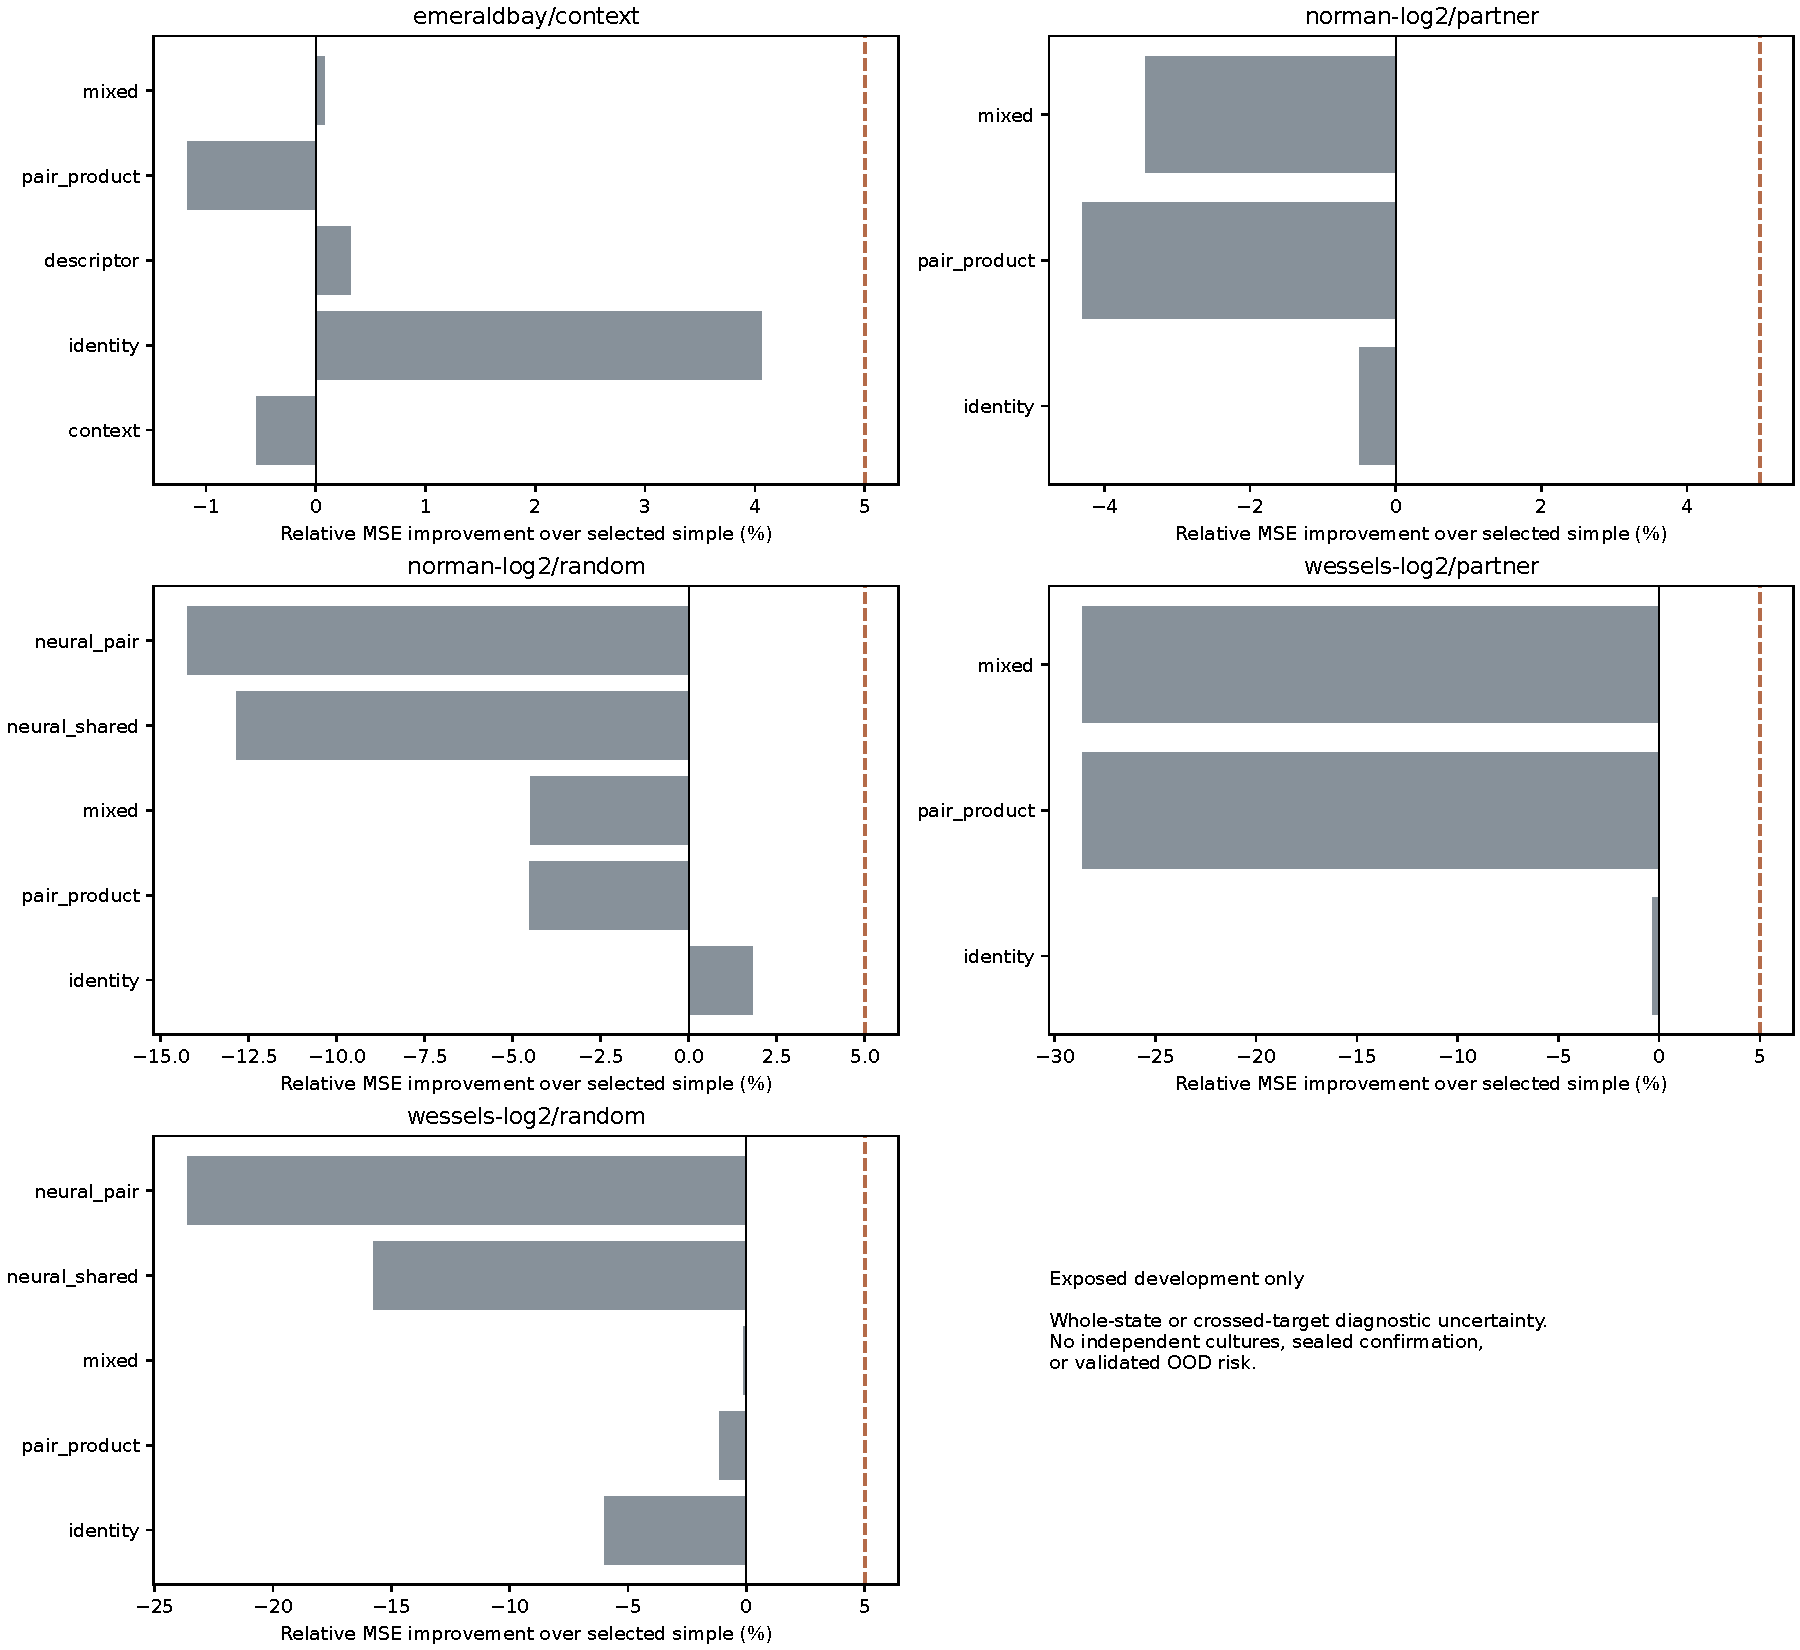
\includegraphics[width=\linewidth]{evidence/stage1_results.pdf}\caption{Information, pair attribution and neural changes against retained simple competitors. The dashed line is the registered development materiality screen.}\end{figure}

\begin{figure}[htbp]\centering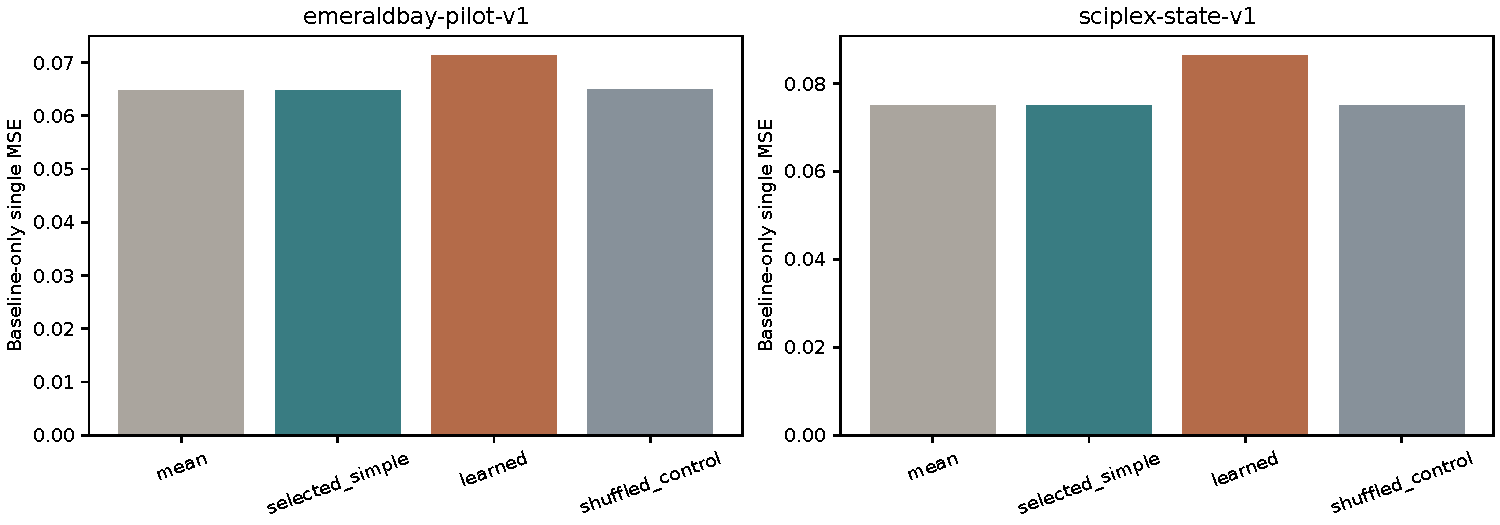
\includegraphics[width=\linewidth]{evidence/stage1_main.pdf}\caption{Separate baseline-only main prediction with fixed source identity support. Shuffled-control results are fixed-selection sensitivities.}\end{figure}

Independent joint transfer remains unevaluable. It requires globally held pair identities, multiple sealed pretreatment states, independently initiated cultures with matched controls and singles, and declared query-reference adaptation. Reliability, acquisition and scaling remain conditional.
